\documentclass[12pt]{article}
\usepackage[a4paper]{geometry}
\usepackage[myheadings]{fullpage}
\usepackage{amsmath,amssymb,amsthm, enumitem, hyperref, tabto} 
\usepackage{fancyhdr}
\usepackage{arxiv}
\usepackage{lastpage}
\usepackage{graphicx, wrapfig, subcaption, setspace}
\usepackage[font=small, labelfont=bf]{caption} \usepackage{blindtext}
 \usepackage{blindtext}
\usepackage{url, lipsum}
\usepackage{tgbonum}
\usepackage{amsmath,physics}
\usepackage{authblk}
\usepackage{hyperref}
 \hypersetup{ 
     colorlinks=true, 
     linkcolor=blue, 
     filecolor=blue, 
     citecolor =red,       
     urlcolor=cyan,
     pdftitle={Noisy Student Training to identify Textual Elements in Unsupervised News Data via Argumentative Essay Pieces}
     } 
\usepackage[super,compress,sort,numbers]{natbib}
\usepackage{csquotes}
\usepackage{multicol}
%\setlength{\multicolsep}{6.0pt plus 2.0pt minus 1.5pt}% 50% of original values
\usepackage{xcolor}
\usepackage{algpseudocode}
\usepackage{algorithm}
\floatname{algorithm}{Algorithm}
\usepackage{times}
\usepackage{adjustbox}
\usepackage[T1]{fontenc}
\usepackage{makecell}
\usepackage{parskip}
\usepackage{erewhon}
\usepackage{geometry}
\usepackage{caption}
\usepackage{subcaption}
\usepackage{framed}
\setlength\FrameSep{0.5em}
\setlength\OuterFrameSep{\partopsep}
% \usepackage{draftwatermark}
\graphicspath{ {./images/} }
\usepackage{sectsty}

\sectionfont{\fontsize{15}{20}\selectfont}
\usepackage{tikz}
\def\checkmark{\tikz\fill[scale=0.4](0,.35) -- (.25,0) -- (1,.7) -- (.25,.15) -- cycle;} 
\usepackage[sorting=none]{biblatex}
\addbibresource{references.bib}

\newcommand{\HRule}[1]{\rule{\linewidth}{#1}}
\onehalfspacing
\setcounter{tocdepth}{5}
\setcounter{secnumdepth}{5}

\renewcommand{\headrulewidth}{0pt}
\renewcommand{\footrulewidth}{0pt}

\begin{document}

% \SetWatermarkText{RO014-Embodied AI for computational perception and understanding of spatial designs-Karimi Zayan, Prannaya Gupta}
% \SetWatermarkColor[gray]{0.5}
% \SetWatermarkFontSize{0.35cm}
% \SetWatermarkAngle{0}
% \SetWatermarkHorCenter{12cm}
% \SetWatermarkVerCenter{1cm}


\pagestyle{fancy}
\fancyhf{}
\fancyhead[L]{\footnotesize \textbf{CS5131} Project - \emph{Noisy Student Training to identify Textual Elements in Unsupervised News Data via Argumentative Essay Pieces}}
\fancyhead[R]{\footnotesize \emph{Liew Wei Pyn, Prannaya Gupta}}
\fancyfoot[R]{Page \thepage\ of \pageref{LastPage}}


{\selectfont
\title{
	\huge \textbf{Noisy Student Training to identify Textual Elements in Unsupervised News Data via Argumentative Essay Pieces}
}

\date{}

%\author{\LARGE \textbf{RO014}}

\author[1]{Liew Wei Pyn}
\author[1]{Prannaya Gupta}
\affil[1]{NUS High School of Math and Science}

\maketitle



\begin{abstract}
\emph{Noisy Student Training and Knowledge Distillation are separate techniques to boost the accuracy and noise-resistance of a given model. Although largely used on Convolutional Neural Networks (ConvNets), prior work has show their legitimacy on Natural Language Processing (NLP) tasks and specifically transformers. We design a system inspired by these techniques to craft a robust model capable of identifying textual elements in argumentative essay pieces and news pieces (particularly opinion editorials), such as the Lead, Position and Concluding Statement. Initially, we use transfer learning on multiple pretrained models retrained on a set of argumentative essays to get a set of Teacher models, after we apply selection and then follow through with data augmentation through word and sentence-based augmentation. Sequences are labelled by a teacher model and the labelled data is passed into a student model based on the RoBERTa architecture, with Layerdrop and dropout implemented, which is now retrained again to produce a student model, which repeatedly replaces the teachers and the steps take place again iteratively, allowing a set of comparable student models. We compare and contrast to find the best model capable of identifying these essays. A User Interface is later designed to visualise these models separately.} \\
\begin{flushright}(215 words)\end{flushright}
\end{abstract}

\thispagestyle{empty}

\newpage

\tableofcontents

\thispagestyle{empty}
\newpage

\section{Introduction}

Argumentative Essays are one of the key ways by which a student's calibre in language is assessed. Generally, this quantity is assessed based on a hour to one-and-a-half hour paper that prompts the student with any $n$ topics. These topics are based on key sociopolitical concepts, bordering on current affairs topics such as the recent Covid-19 Pandemic. These essays have many different forms, but there is often a key format, as highlighted in the diagram below:

\begin{framed}\noindent
        \textbf{Lede (Lead)}: Introductory paragraph introducing the concepts, context and definitions held in the entire essay, in an engaging manner. \\
        
        \textbf{Thesis (Position)}: Indication of author's point of view, summarising key points highlighted in the essay. \\
        
        \textbf{Point (Claim)}: Usually statements not yet justified based on data or elaboration which are raised at the start of a body paragraph. \\
        
        \textbf{Evidence, Explanation, Examples, Elaboration (EEEE)}: Statements based around relevant facts and case studies justifying one's point. \\
        
        \textbf{Counterargument (Counterclaim)}: Statements highlighting opposing points of view from other perspectives and onlookers. Usually start with something like \textit{"Critics may say..."} or \textit{"Some may argue that..."}. \\
        
        \textbf{Rebuttal}: A rebuttal aims to refute the point raised in a Counterargument, reaffirming the Position of the author.
        
        \textbf{Conclusion (Concluding Statement)}: The author delivers some call for action or some other smaller points to iron out his Position clearly to anyone reading.
\end{framed}

Argumentative Essays usually include a plethora of these different essay elements that are quite difficult for the average student to identify.

For instance, given this passage, taken from Leemen Chan et al:

\begin{displayquote}
\emph{Although the history of human invention spans over millennia, there have been relatively few game-changing technologies. From the manipulation of fire back in the primal age to the invention of the electronic transistor in the 1940s, these monumental developments have often been followed up by fervent exploration and a burgeoning of new technologies that stem from that initial spark.}
\end{displayquote}

Here, you can state that this paragraph is the Lede, or the \textbf{Lead}. It is the statement of facts prior to a statement of opinion, and this is a very objective set of statements.

However, after this, the author writes the following:

\begin{displayquote}
\emph{While some may say Artificial Intelligence, or AI, is akin to these other inventions, I beg to disagree.}
\end{displayquote}

This is a \textbf{Position}, as can be said from the subjective statement of opinion, which has yet to be substantiated by fact or evidence. However, in a different context, this can be classified as a \textbf{Rebuttal} as well, since it started by giving an alternate perspective and then admitting that this is not something that matches up with the perspective of the author. The fact is that this Position is identified based on the context laid out by prior sentences.

This contradiction can often cause confusion in modern machine learning models, since they may classify sentences without keeping track of context. Context is quite important in Natural Language Processing (NLP) Tasks, which is something many models would not excel at.

Often, students struggling with or generally writing essays use automated writing feedback tools, which, while numerous, each have their own limitations. Many of these feedback tools are unable to identify writing structures in essays, or are at least very inaccurate in their identification. Many of these tools are proprietary, with algorithms and feature claims that cannot be backed up independently, and more importantly, that are inaccessible to educators and the marginalized populace due to high costs.

In addition, automatically and consistently identifying and highlighting such elements, that too amongst hundreds of scripts, can be a tedious task for teachers, who may wish not to use these tools due to, in summary, their high levels of inaccuracy, lacking features and high costs.

Hence, our aim with this project is to develop a model capable of analysing and identifying the key argumentative elements in an English essay or even a news article\footnote{You can find our Research Repository at \url{https://github.com/treeai/writingAnalysis}}. We target the Minimum Viable Product (MVP)\footnote{You can find our MVP Repository at \url{https://github.com/treeai/writingAnalyzer}}, particularly a Web User Interface (UI), designed post-modelling to be aimed towards teachers aiming to help their students improve their writing, and students aiming to improve their writing to prepare for the A Level General Paper and University Applications Preparation.


%\newpage

\section{Methodology}

\subsection{Data Collection}

\subsubsection{The Feedback Prize Dataset}
\label{section:feedbackprize}
The Feedback Prize Dataset~\cite{feedbackprize} is a textual dataset containing roughly 60,000 samples of argumentative essays written by U.S students in grades 6-12. These essays have been annotated by expert raters for elements commonly found in argumentative writing. Provided by the Georgia State University in a partnership with the Learning Agency Lab, this dataset focuses primarily on student writing, and, having been labelled, is a much better candidate to use with Deep Supervised Learning. This dataset has been retrieved from the Kaggle Competition, "Feedback Prize - Evaluating Student Writing".

A sample of the essay (partial) is shown below:
\begin{displayquote}
\textit{Asking multiple people for advice can very heavily influence how you may act on certain topics. Receiving advice from multiple people is not such a bad thing as it may seem. Receiving advice from multiple people is good because it can influence your decision, teach you more about the topic, and more points of view on the topic.}

\textit{Getting more peoples' opinions can heavily impact your decision. Having more opinions means more choices you can choose. This means that the more options you have, the easier it is to do the right thing. Others' opinions can stop you from doing the wrong thing. When they tell you their end it may impact you and stop you from doing something you wouldn't have wanted to do. Others' opinions can also show you what consequences there might be for your actions. They might tell you the possibilities of what might happen when you say that. People opinions can greatly impact what you do.}

\end{displayquote}

\subsubsection{The New York Times Article Database}
\label{section:nytimes}

\begin{figure}[!ht]
    \begin{center}
        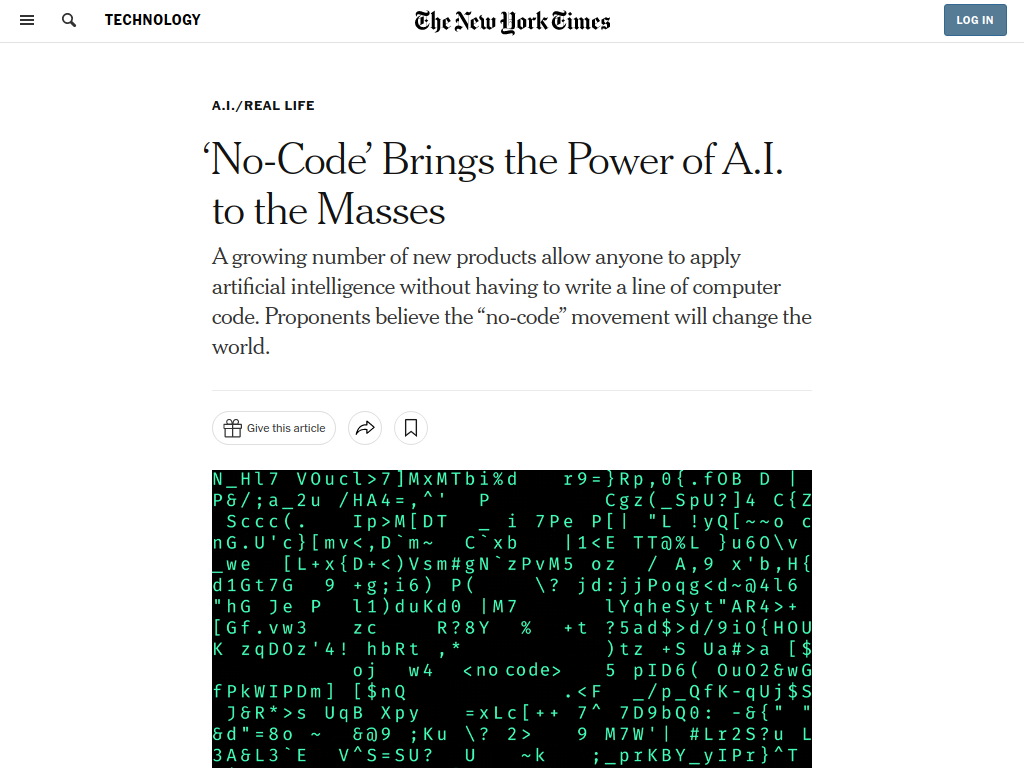
\includegraphics[scale=0.3]{images/nytimes_example.png}
        \caption{An example of an article considered for this project.}
        \label{fig:nytimes_example}
    \end{center}
\end{figure}

Whilst it is agreeable that the Feedback Prize Dataset (\ref{section:feedbackprize}) is a suitable choice for training, given the fact that is labelled and, in that way, a pretty unique dataset, the essays are also made up of a relatively broken form of English, given the fact that they are written by younger individuals, hence it possesses quite a bit of noise within the textual samples. The samples are also not ideal for models that are not necessarily very noise-resistant, hence The New York Times Article Database is retrieved for noise removal.

The New York Times Article Database is used to introduce relative noise in terms of the variety of samples, while also sticking to perfect English (since it is a publication). Data is retrieved based on a dynamic set of New York Times article URLs, which is also retrieved programmatically from every topical section referenced in their website. The article texts, in addition to the title, are stored into a database, and the articles are filled within a set of text files in a similar format to the aforementioned Feedback Prize Dataset. There are no labels available for this dataset, and our teacher model will address this issue later. Just as a note, this database is made of texts, not separated into sentences. Hence, NLTK's~\cite{nltk} \texttt{PUNKT} Sentence Tokenizer~\cite{punkt} is used to segment the articles into sentences.

\subsection{Algorithms Employed}

\subsection{The Transformer}
The transformer is a well known model architecture introduced by Vaswani et al.\cite{transformer} to solve a variety of NLP tasks. Because the use of transformers is commonplace and our implementation does not deviate from traditional transformer architectures, we will omit an exhaustive description of the transformer, and instead refer readers to the incredibly informational resources such as the original paper \cite{transformer} and online guides such as The Annotated Transformer. \footnote{\url{http://nlp.seas.harvard.edu/2018/04/03/attention.html}}


\begin{figure}
     \centering
     \begin{subfigure}[b]{0.3\textwidth}
         \centering
         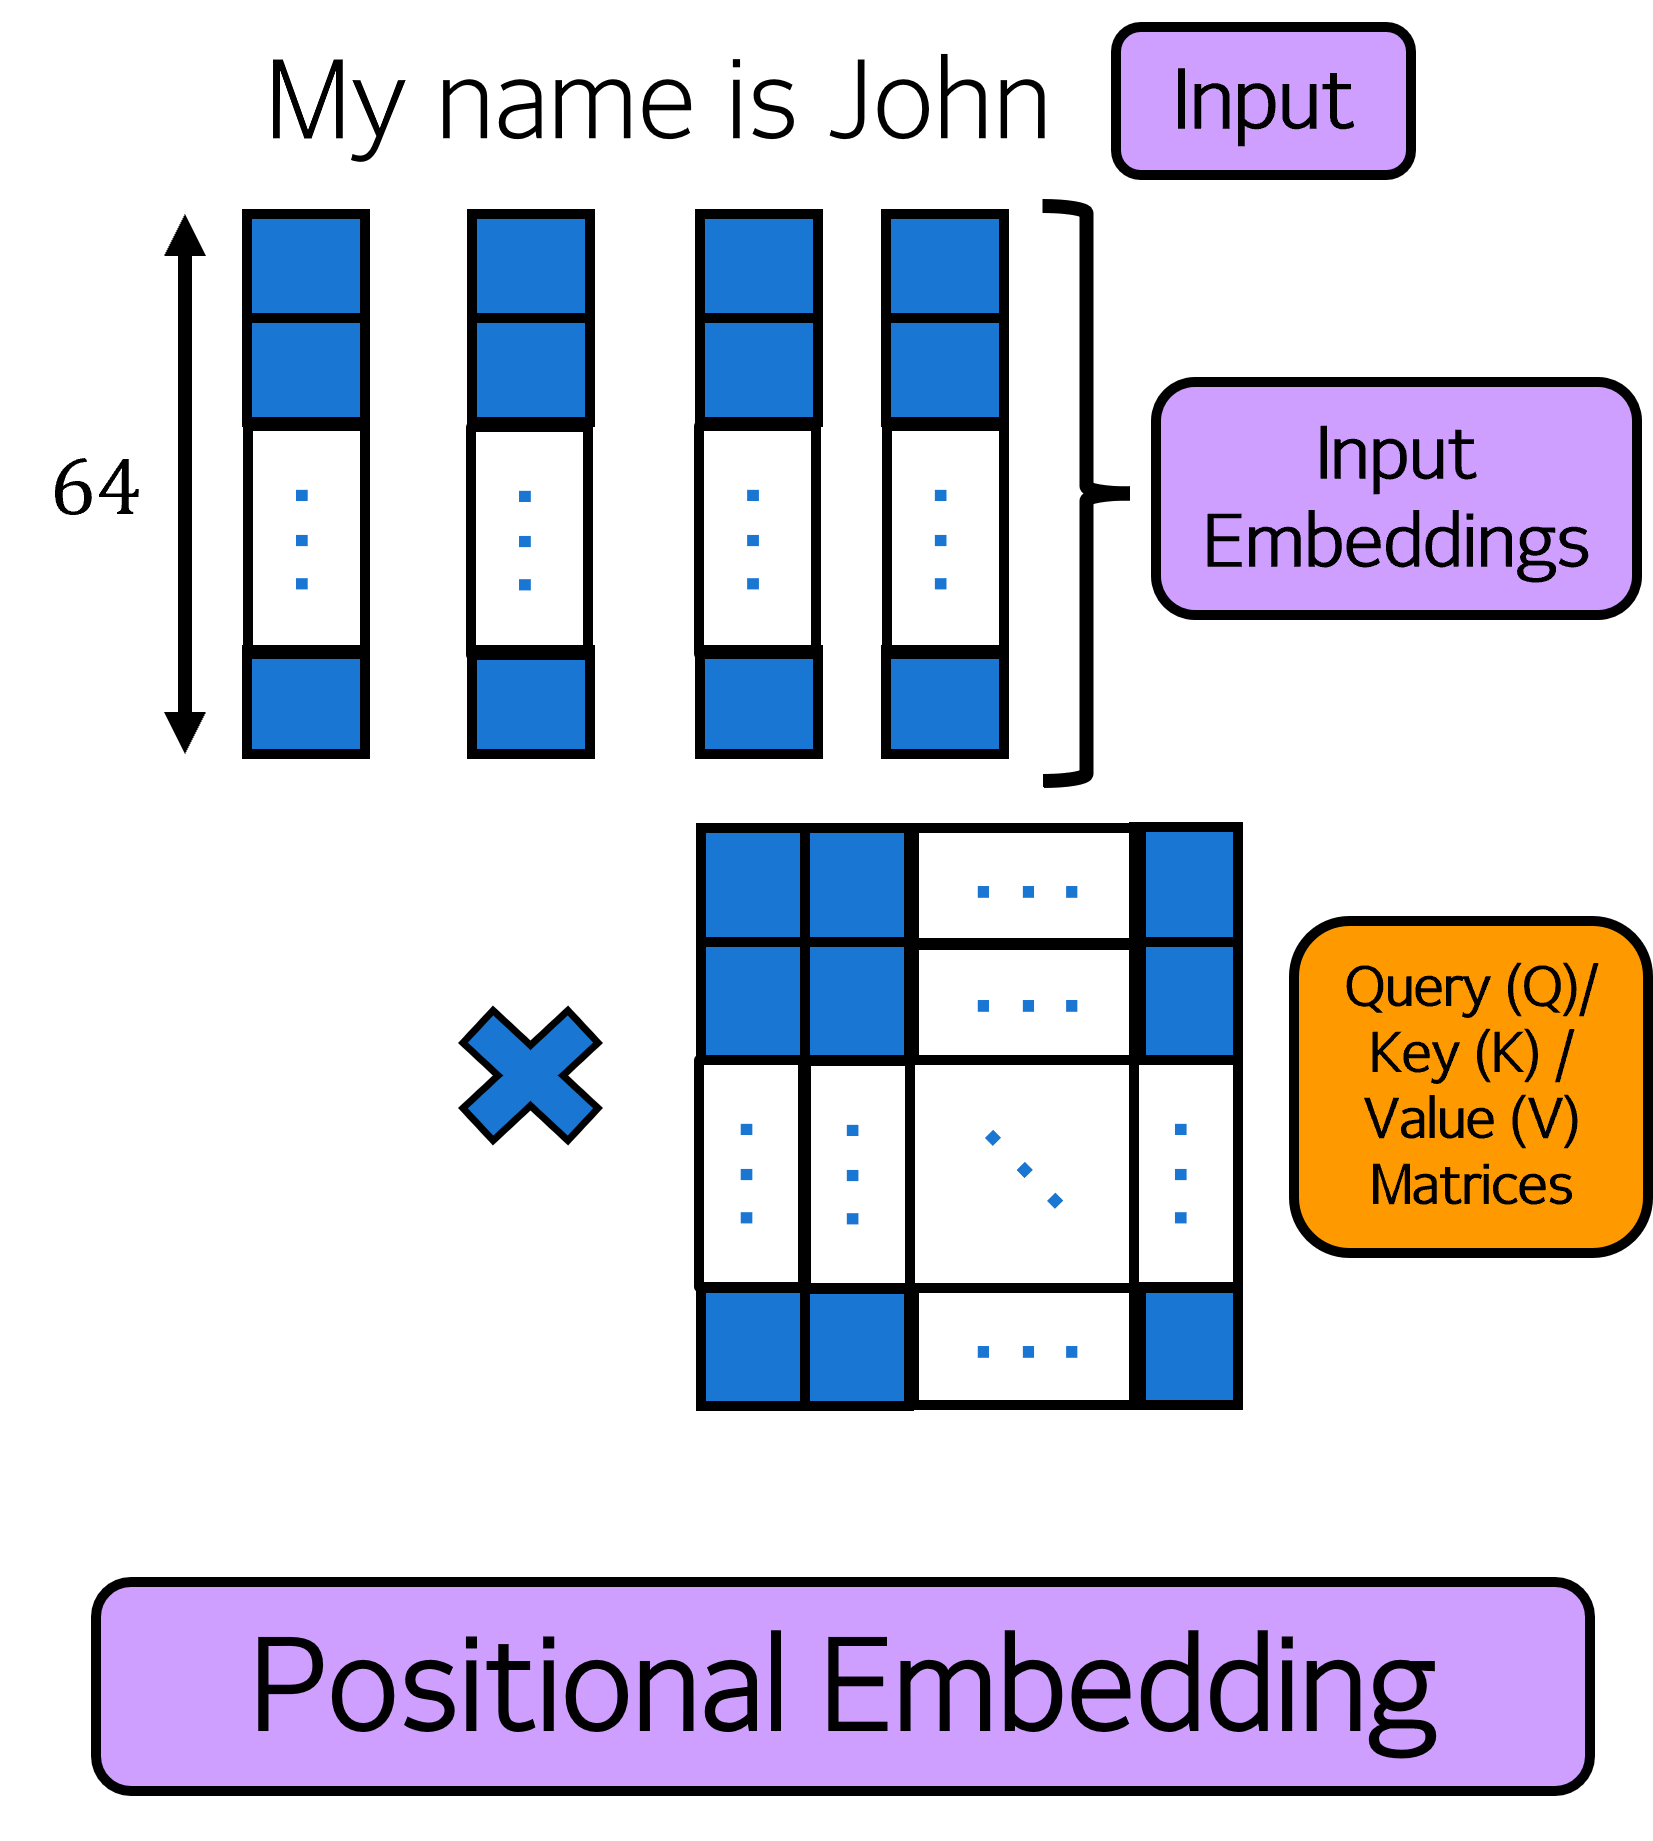
\includegraphics[width=\textwidth]{images/inputting.png}
         \caption{A representation of the embedding done by transformers.}
         \label{fig:transformer_input}
     \end{subfigure}
     \hfill
     \begin{subfigure}[b]{0.3\textwidth}
         \centering
         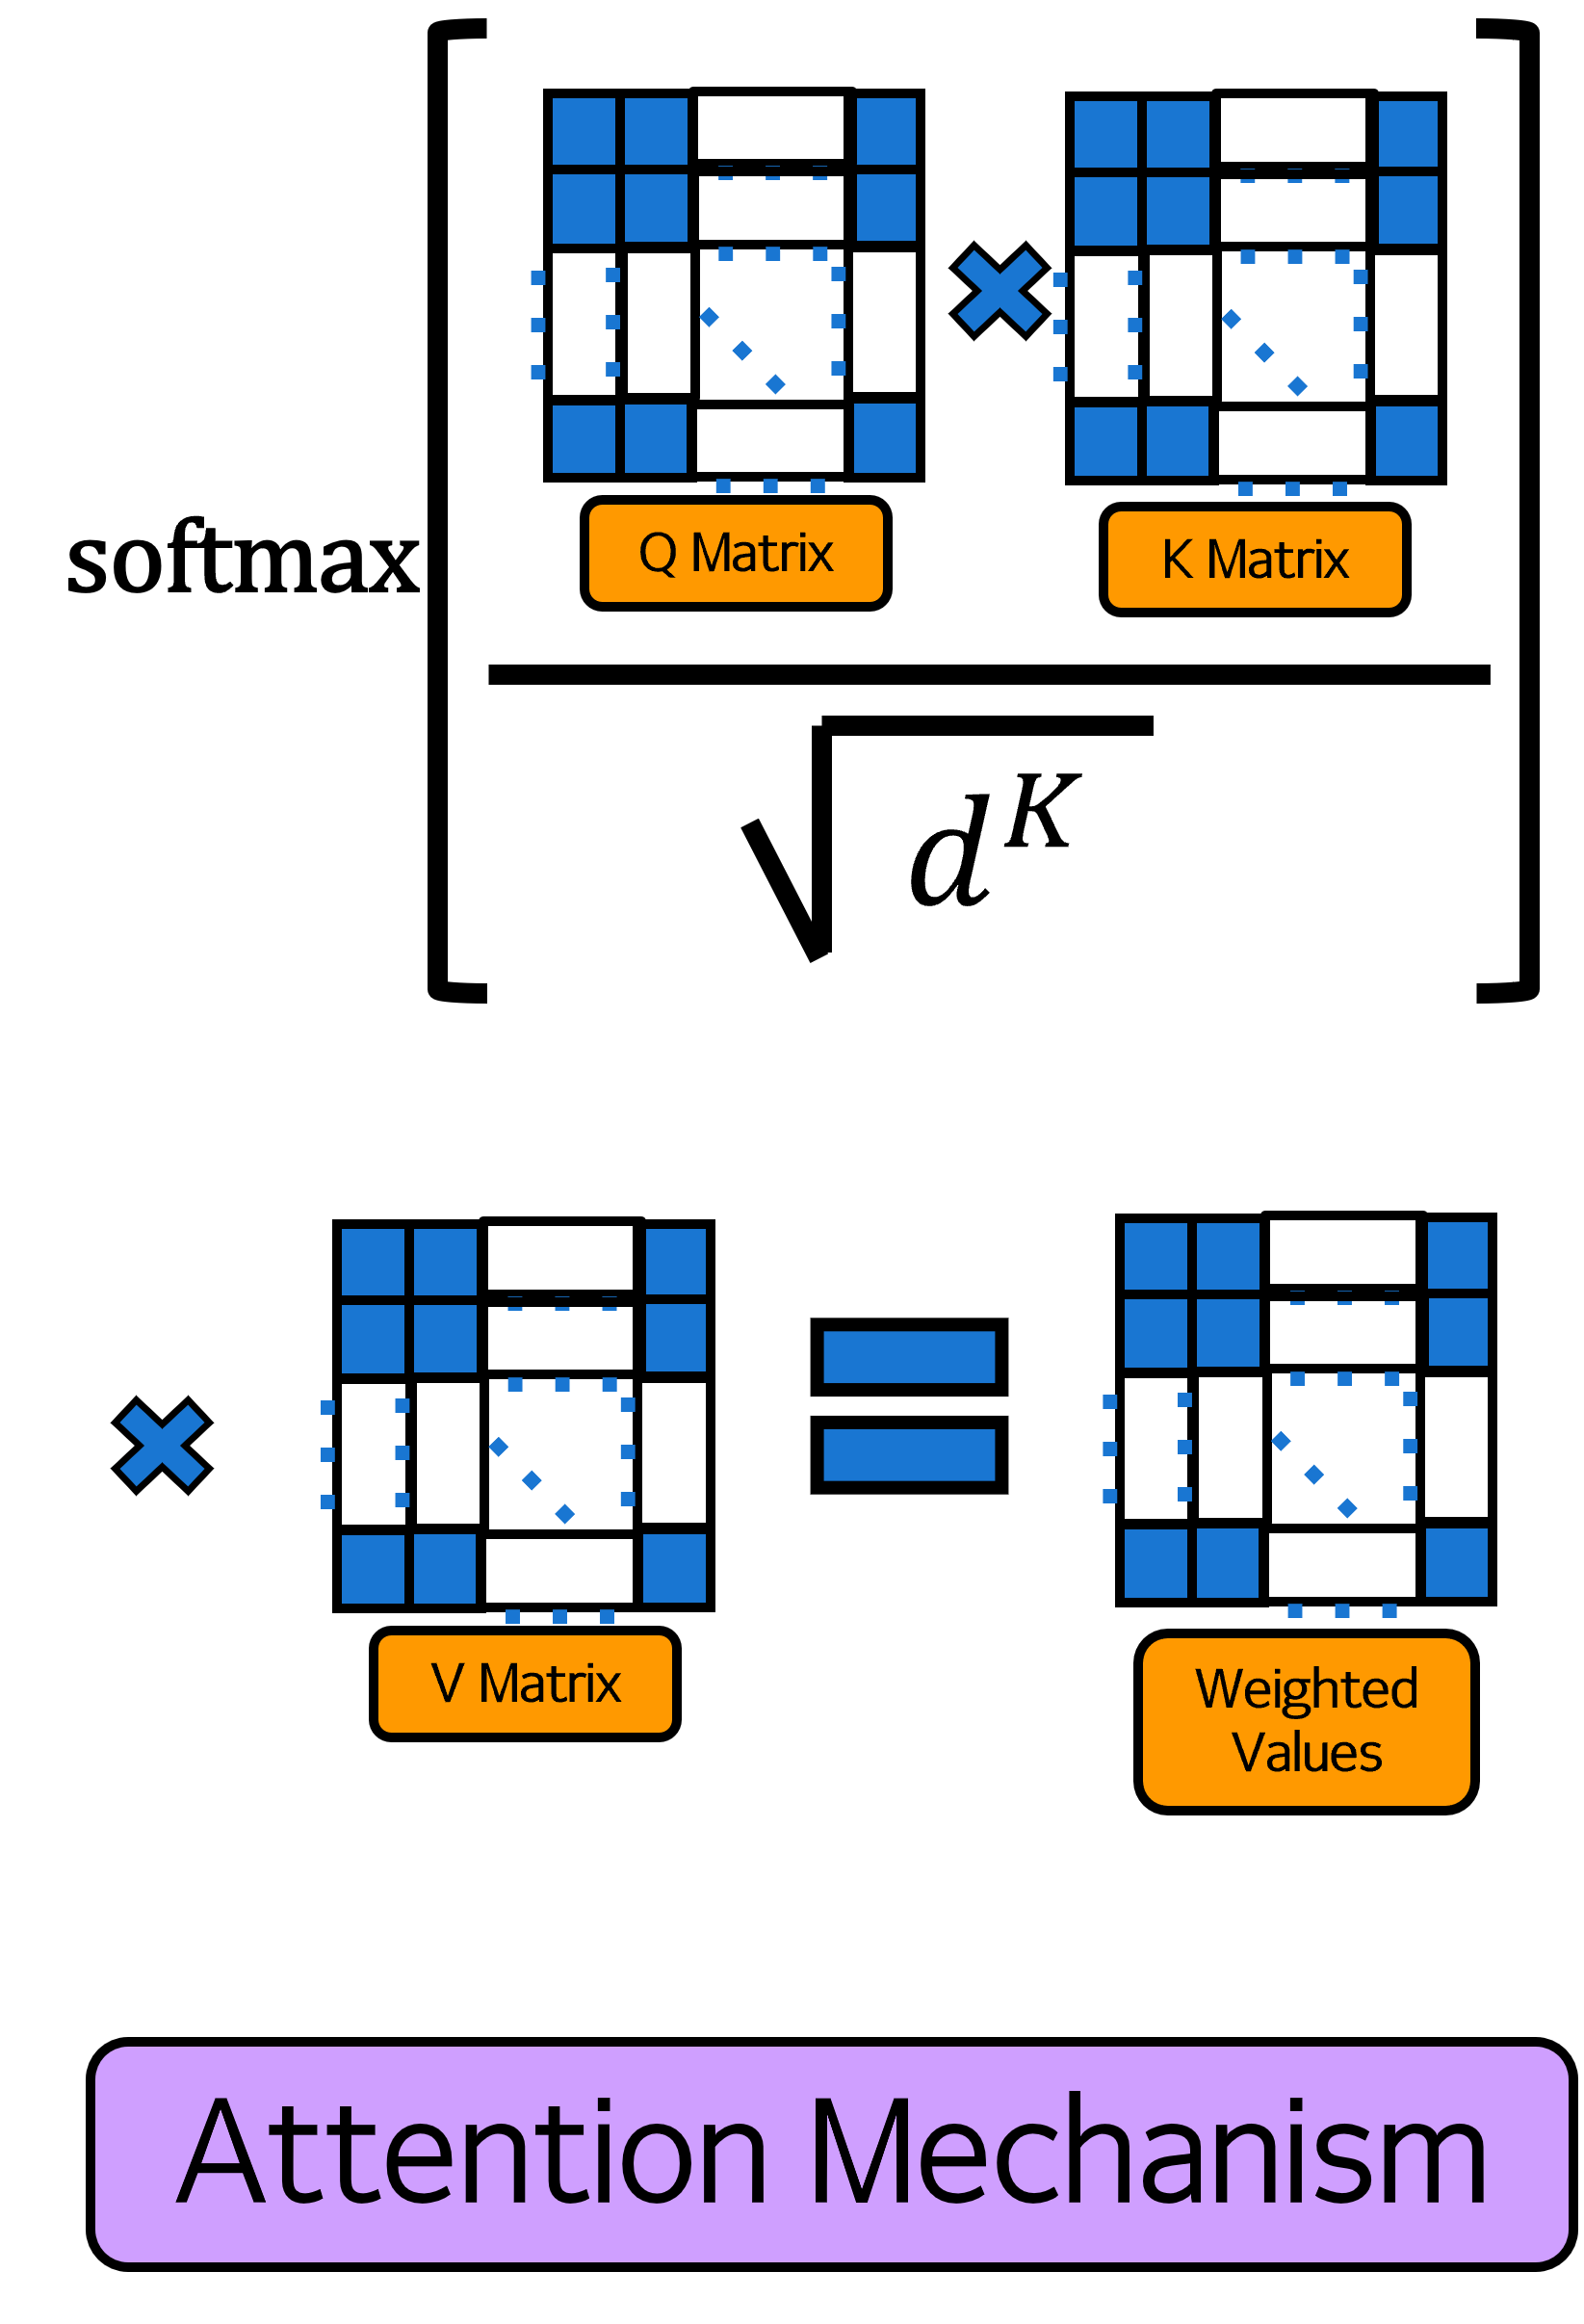
\includegraphics[width=\textwidth]{images/attention.png}
         \caption{A representation of the attention layers in transformers.}
         \label{fig:attention}
     \end{subfigure}
     \hfill
     \begin{subfigure}[b]{0.3\textwidth}
         \centering
         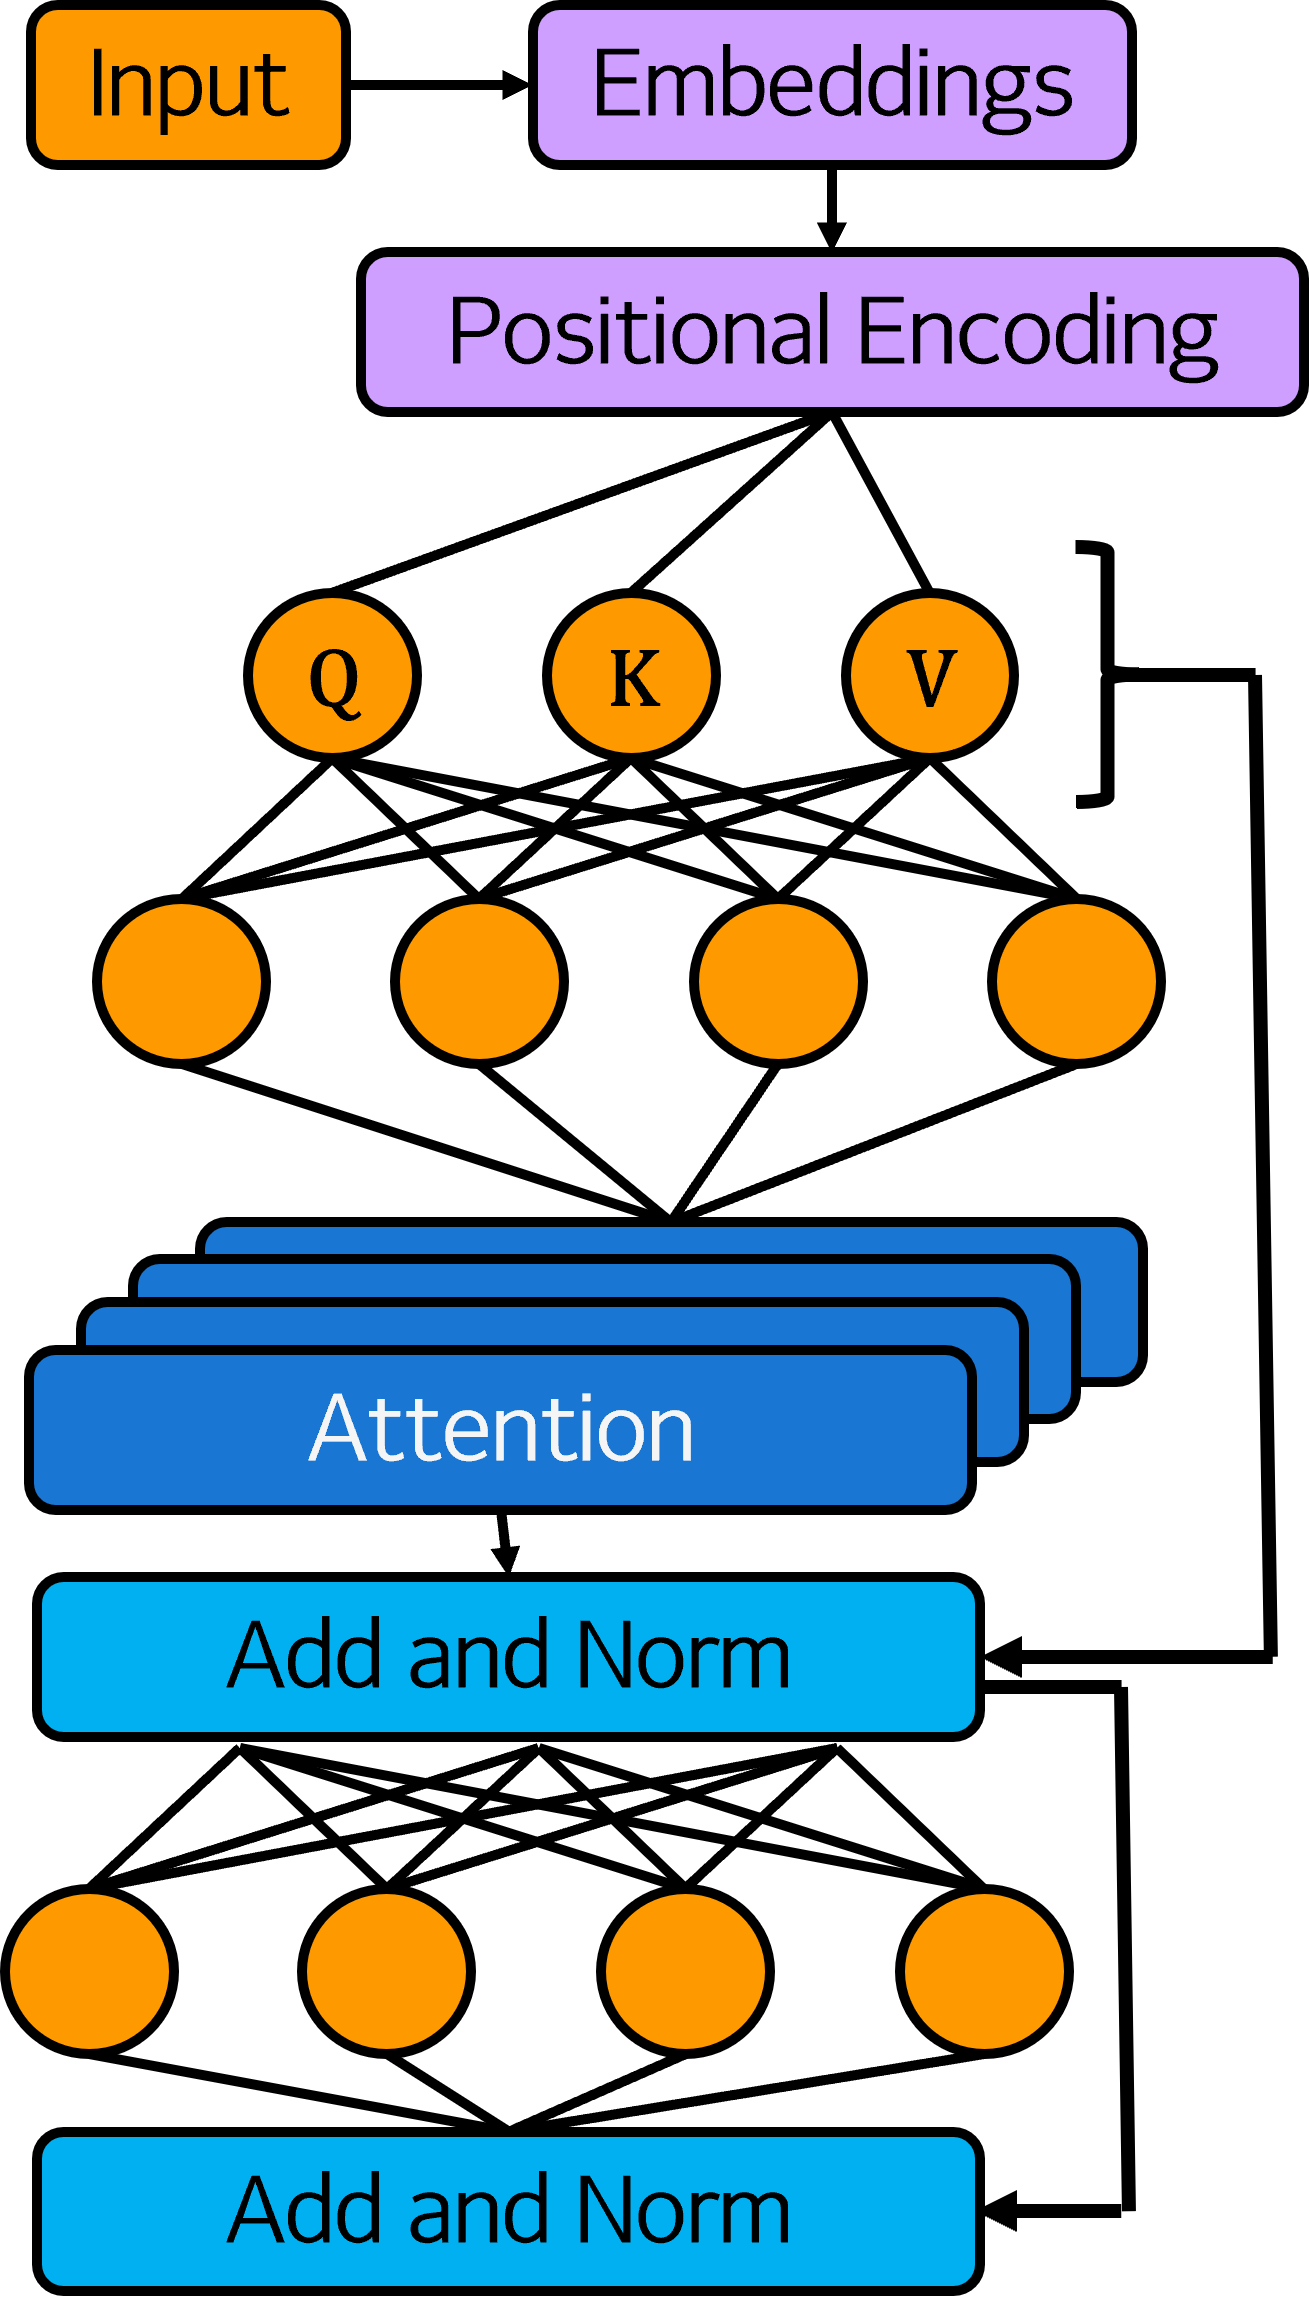
\includegraphics[width=\textwidth]{images/transformer.png}
         \caption{The overall process of the encoder in a transformer.}
         \label{fig:transformerencoder}
     \end{subfigure}
        \caption{Three simple graphs}
        \label{fig:three graphs}
\end{figure}


\subsubsection{LayerDrop}

Stochastic Depth is a technique initially introduced by Huang et al.~\cite{stochasticdepth} to accelerate training of very deep ResNets~\cite{resnet} for image tasks with depth well beyond 1200 layers. During training time, a random subset of layers are dropped and bypassed, while the entire deep network is used during inference time. This reduces training time substantially as well as improves test error significantly by reducing gradient vanishing and diminishing forward flow. 

Inspired by work on Stochastic Depth, the LayerDrop technique was introduced by Fan et al.~\cite{layerdrop}, applied to transformers for sequence modelling tasks. While Stochastic Depth is interested in accelerating the training of very deep ResNets, LayerDrop intends to reduce the final model complexity of transformers. Utilising the same principle of structured dropout of layers in the encoding and decoding blocks of the transformer during training time, the authors found that the transformer models became more resistant to predicting with missing layers, and they were able to prune the larger model during inference time to obtain a smaller sub-network from any depth without fine-tuning with limited impact on performance.

We note that this metric applies to residual layers (depicted with the function $\mathcal{R}$), which can be formally defined as shown below:
\[ x_{i+1} = x_i + \mathcal{R}(x_i) \]
In LayerDrop, a drop rate, $p^* \in [0, 1]$, is introduced, based on a set of $N$ groups and pruning set of $r$ groups, based on the following definition:
\[ p^* = 1 - \frac{r}{N} \]
On general principle, $p^*$ is set to be either $0.2$ ($r = 0.8 \cdot N$) or $0.5$ ($r = 0.5 \cdot N$), although Fan et al~\cite{layerdrop} suggests using $p^* = 0.5$ for models aimed for small inference-times.

Now you define a variable $Q_i \in \{0, 1\}$ which represents a Bernoulli Distribution similar to dropout, which is used to ascertain whether or not to skip or use the layer. $Q_i$ is dictated by the following equations (by Wang et al~\cite{layerdrop2}):
\begin{align*}
    P(Q_i = 0) &= p \implies P(Q_i = 1) = 1 - p \\
    x'_{i+1} = x_i &+ Q_i \times \mathcal{R}(x_i)
\end{align*}

\subsubsection{Knowledge Distillation and Expansion}
Knowledge Distillation~\cite{knowledgedistillation} refers to the process where a larger, difficult to deploy model transfers its learned knowledge about its task to a smaller, faster model. This is typically used to reduce large sized models into computationally less expensive models for real-world deployment. The larger model is often termed the "teacher" model, and the smaller model the "student". Existing work done in the field of knowledge distillation for NLP is limited and focuses on feature-basead knowledge, wherein the student model tries to replicate the feature embeddings (intermediate layers) of the teacher model. This includes work done by Shin et al.~\cite{TSembeddingdistillation} wherein they use knowledge distillation and ensemble methods for word embedding distillation, as well as Jiang et al.~\cite{KDberttospeech} that demonstrates knowledge distillation from pretrained BERT models achieves improvements in performance. 

In related work in the usage of teacher student models for images, Xie et al.~\cite{noisystudent} introduces the semi-supervised Noisy Student training approach, demonstrated on ImageNet~\cite{imagenet}, which while similar to Knowledge Distillation in terms of utilising soft labels and the teacher student model, has some key differences. Knowledge Distillation focuses on model compression, without use of unlabelled data or noise injection. On the contrary, Noisy Student makes use of unlabelled data, noise injection and student models that are not smaller than the teacher model. The authors describe their approach intuitively as "knowledge expansion", where they enable the student model to outperform the teacher model.

\begin{figure}[!ht]
    \begin{center}
        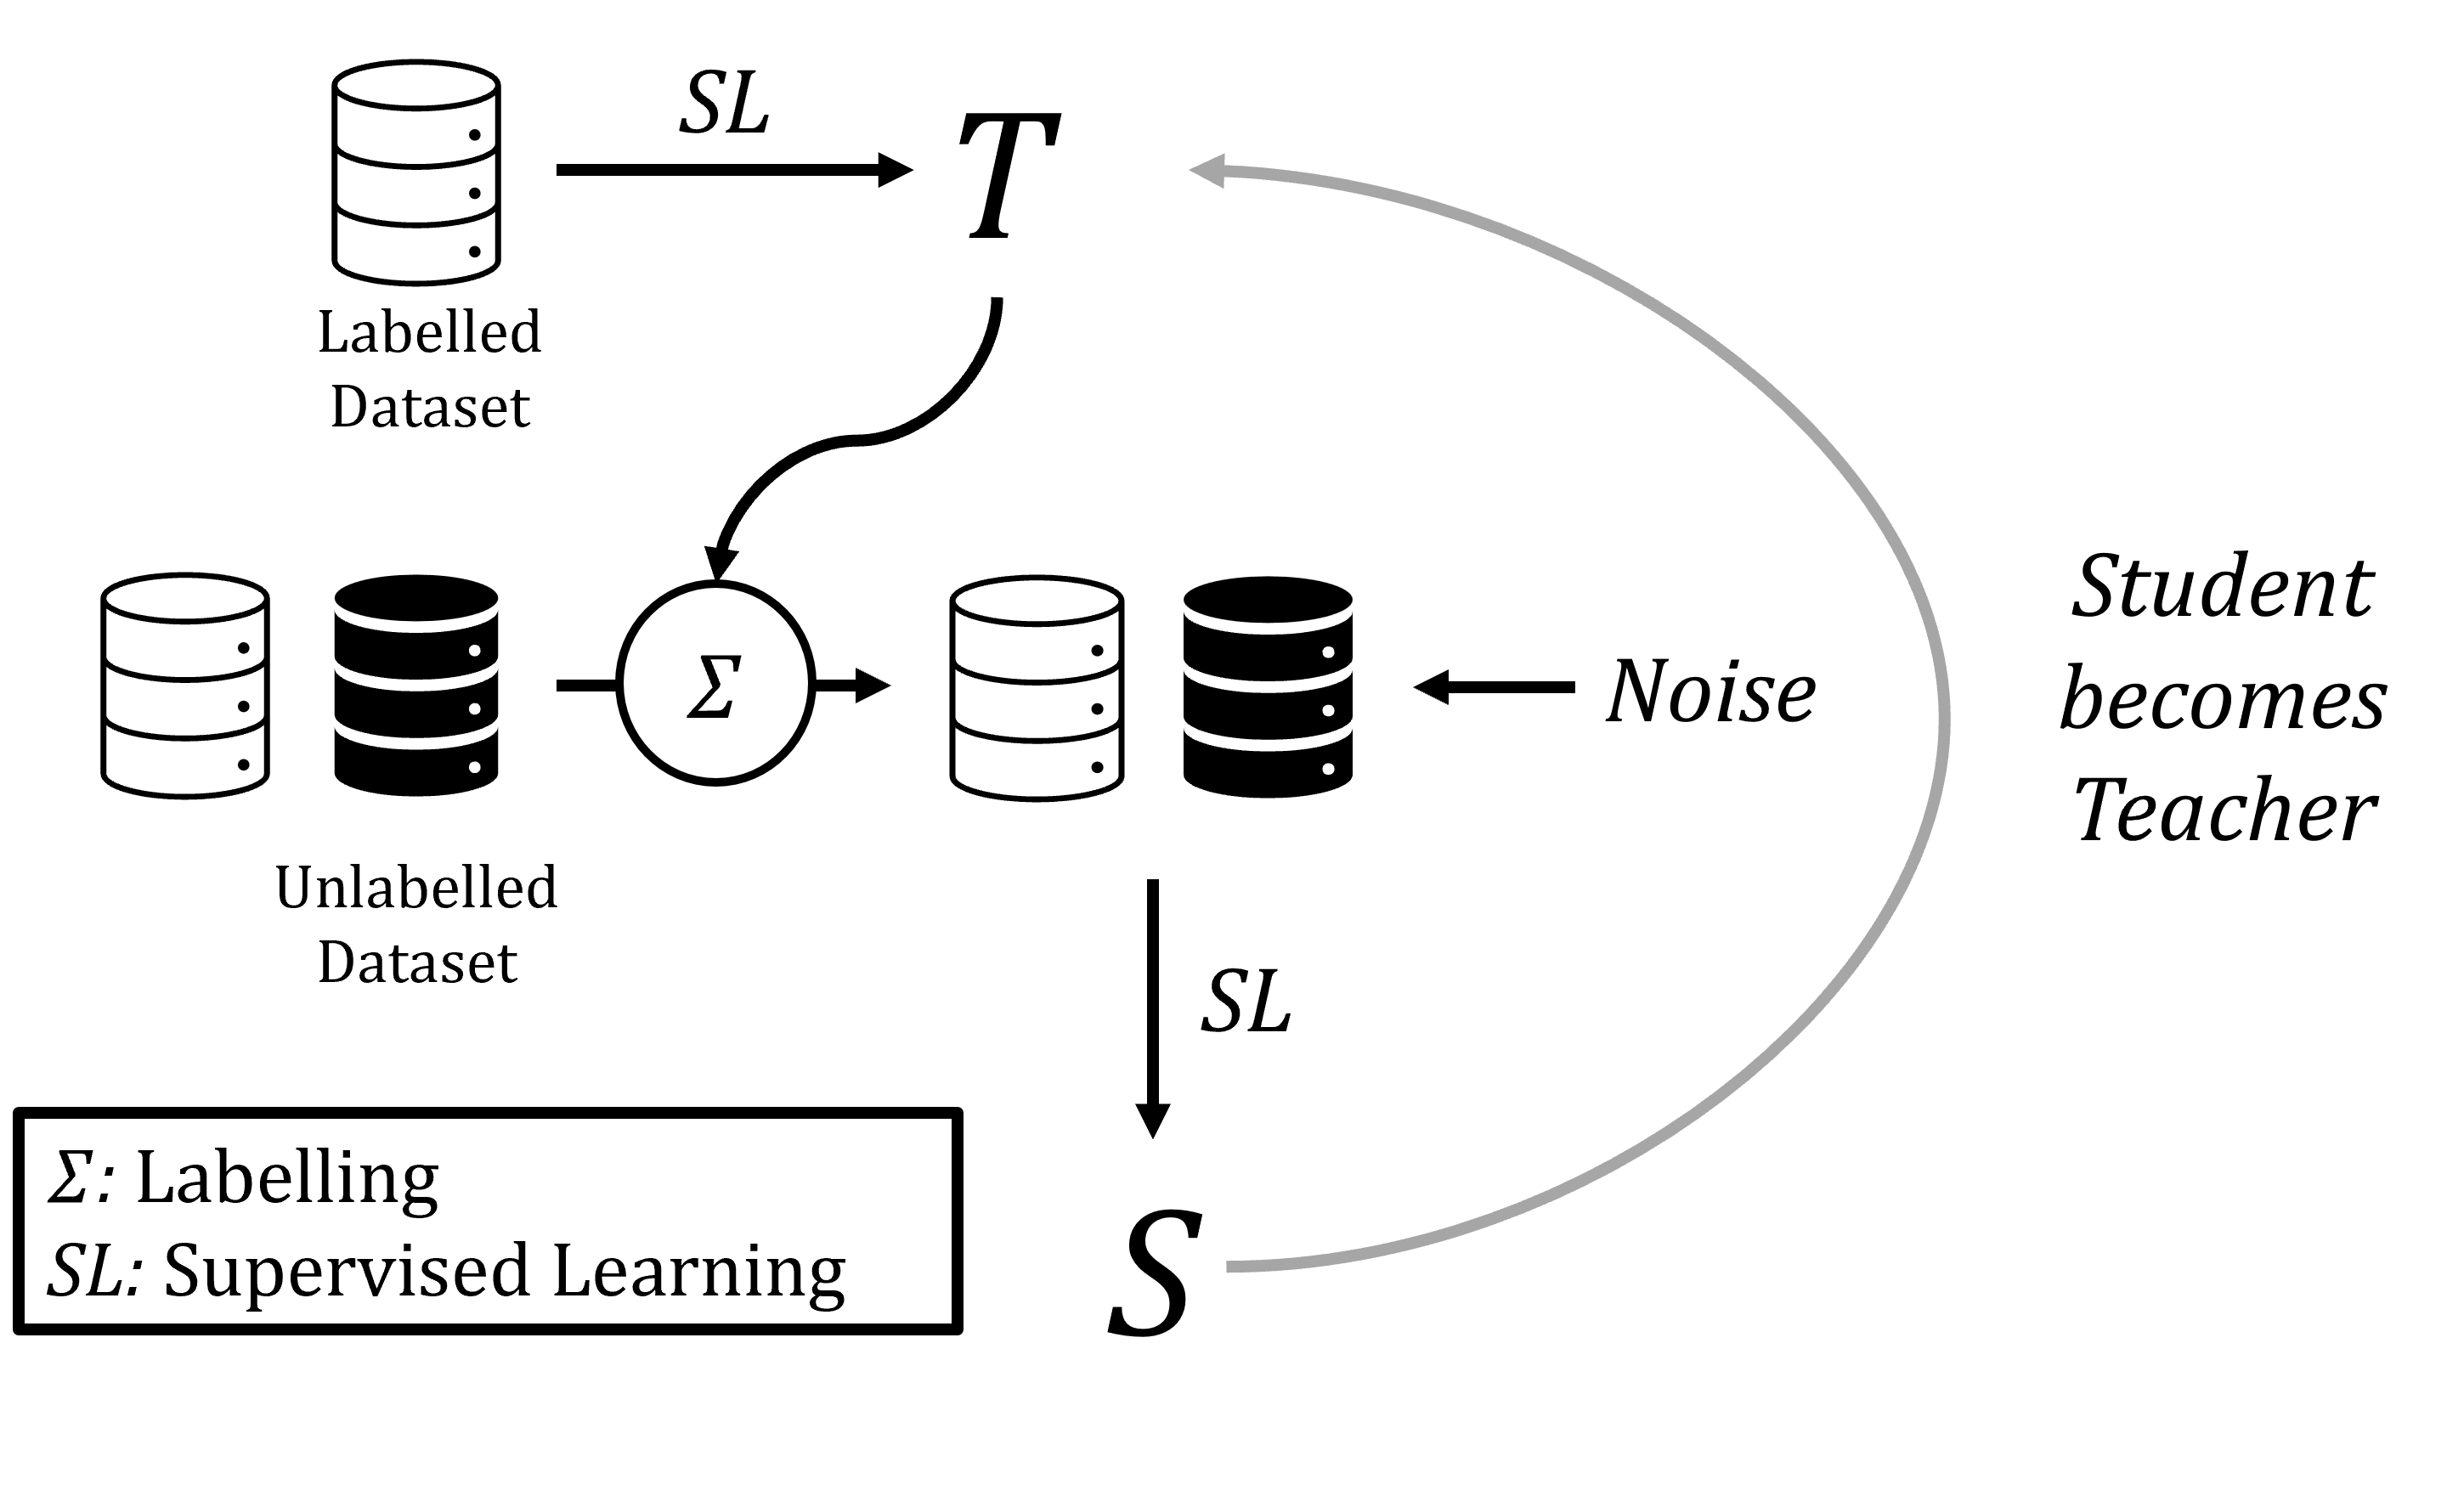
\includegraphics[scale=0.5]{images/noisy_student.png}
        \caption{How Noisy Student Training works.}
        \label{fig:noisystudent}
    \end{center}
\end{figure}

Noisy Student injects noise into the dataset and model through methods highlighted for as follows:
\begin{multicols}{2}
\textbf{Input Noise}
\begin{itemize}
    \item Random Corrupting and Augmentation
    \item Mild Rotation
    \item Color/Jitter Changes
\end{itemize}
\columnbreak
\textbf{Model Noise}
\begin{itemize}
    \item Structured and Unstructured Dropout (skipping of neurons)
    \item Stochastic Depth (skipping of residual layers)
\end{itemize}
%\columnbreak
\end{multicols}

Our work expands upon that of Xie et al. in the field of Natural Language instead of Image Classification with some modifications. In terms of input noise, for obvious reasons we cannot rotate natural language (if you find a way do let us know), and we instead perform textual modification via synonym substitution and sentence restructuring. In terms of model noise, we make use of Dropout and LayerDrop~\cite{layerdrop} in place of Stochastic Depth. The use of stochastic depth in this case intends to introduce model noise, and LayerDrop achieves the same effect during training time for the transformer architecture, while additionally allowing us to prune the final student models without major loss in performance. The resulting student models are hence smaller, in contrast to the Noisy Student technique where student models are intentionally larger than the teacher model.


\subsection{Training Process}

\subsubsection{Teacher Model}

A teacher model is obtained based on prior work done on the project. For instance in Xie et al~\cite{noisystudent}, they perform Noisy Student on the previously established EfficientNet model architecture~\cite{efficientnet}. However, due to the relative newness of our dataset, not much prior work has been done to justify using a specific architecture. We instead train both the teacher and student models in order to attain full autonomy, and the teacher model trained is based on much larger models which can gain higher accuracy with ease. We hence utilise the following model architectures:
\begin{multicols}{3}
   \noindent
\begin{itemize}
\item DistilGPT2\cite{distilgpt2}
\item DistilBERT\cite{distilbert}
\end{itemize}
\columnbreak
\begin{itemize}
\item BERT\cite{bert}
\item RoBERTa Base\cite{roberta}
\end{itemize}
\end{multicols}

These are more openly available models derived by researchers from \href{https://ai.google/}{Google AI}, \href{https://ai.facebook.com/}{Meta AI}, \href{https://openai.com/}{OpenAI} and \href{https://huggingface.co/}{Hugging Face} which can be retrained for any specific task. They have been previously pretrained for alternative tasks, and the models are fine-tuned via transfer learning. Transfer learning is a well established technique for improving the performance of machine learning models, and Raffel et al\cite{transferlearningtext} establishes that transformers are no different. Fine tuning transformers trained on rich datasets for downstream tasks achieves state of the art results for dozens of language understanding tasks. Due to their high performance in related language modelling tasks, we utilise these four models and train them using transfer learning.

\begin{figure}[!h]
    \begin{center}
        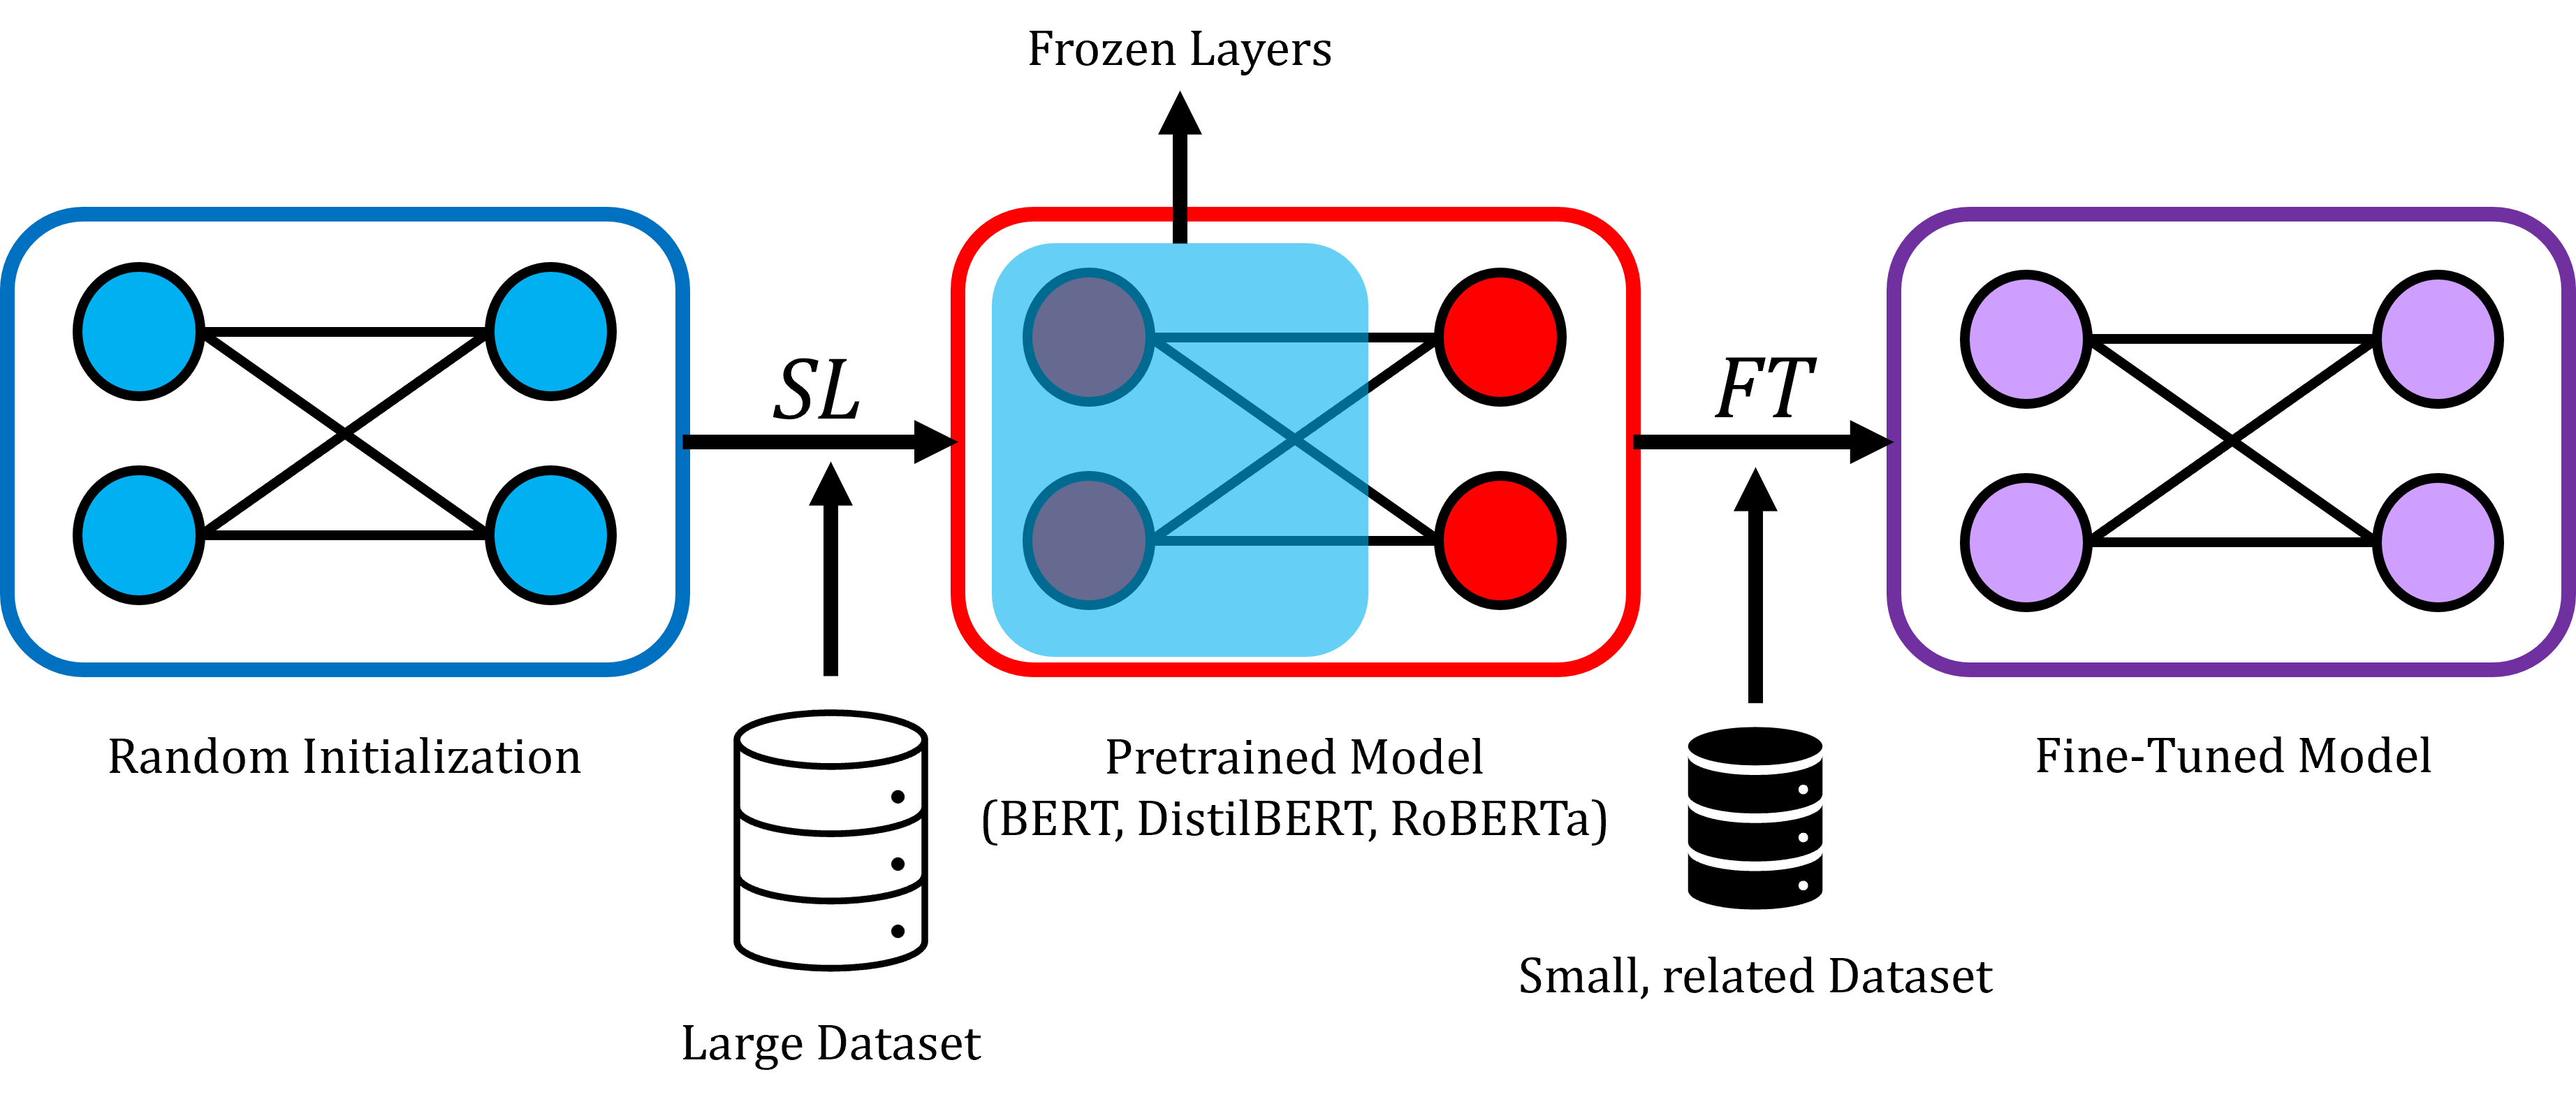
\includegraphics[scale=0.5]{images/transfer_learning.png}
        \caption{How Transfer Learning works.}
        \label{fig:transferlearning}
    \end{center}
\end{figure}

For the selection of the best model, we utilise the following metrics\cite{multiclassmetrics}:
\begin{multicols}{3}
   \noindent
\begin{itemize}
    \item Accuracy
    \item Kappa Coefficient, $\kappa$ \cite{kappa_score}
    \item Precision
    \item Recall
    \item Macro $F_1$ Score\cite{macrof1}
\end{itemize}
\end{multicols}
We use these metrics, in addition to Early Stopping\cite{validation_early_stopping}, to select the best model (and its best epoch) to use as the teacher model going forward.
\subsubsection{Pseudo-labelling and Mock Dataset}
We use the selected teacher model's output logits as soft labels each sample given in the Feedback Prize Dataset (\ref{section:feedbackprize}) and The New York Times Dataset (\ref{section:nytimes}). Instead of relying on one-hot labels, the student model can take advantage of soft labels which contain inherent relationships between classes, helping us a produce a larger mock dataset composed of these pseudo-labelled datapoints. Following Xie et al.\cite{noisystudent} original implementation, when calculating metrics to evaluate model performance on validation split of the datasets, we treat the correct label as the highest probability class predicted by the teacher model.
\subsubsection{Noise Addition}
After this, we inject noise into the given samples. This is done using the \texttt{nlpaug} package~\cite{ma2019nlpaug} which we utilise, with the help of reference to Uribe et al~\cite{nlpaugexample}, wherein \texttt{nlpaug} experiments were carried out to identify ideal forms of data augmentation.

\begin{center}
\begin{tabular}{|c|c|}
\hline \multicolumn{2}{|c|}{\textbf{Contextual Embedding}~\cite{contextual_embedding}} \\
\hline Contextual Word Embedding~\cite{contextual_word_embedding} & Feeding surrounding words to BERT~\cite{bert}, \\ & DistilBERT~\cite{distilbert}, RoBERTa~\cite{roberta} or XLNet~\cite{xlnet, xlnet_gen} \\ & language models to find out the most \\& suitable word(s) for substitution\\
\hline Contextual Sentence Embedding~\cite{contextual_sentence_embedding} & Insert sentence according to XLNet~\cite{xlnet, xlnet_gen},\\ & GPT2~\cite{gpt2, gpt2sentence} or DistilGPT2~\cite{distilgpt2} predictions \\
\hline \multicolumn{2}{|c|}{\textbf{Word-Based Augmentation~\cite{snysubmethod}}} \\
\hline Synonym Replacement~\cite{synonymaug} & Substitute similar word according to \\ & WordNet~\cite{wordnet, wordnetbook} / PPDB~\cite{ppdb, paraphrase} synonym \\
\hline \multicolumn{2}{|c|}{\textbf{Sentence-Based Augmentation~\cite{sentence_aug}}} \\
\hline Abstractive Summarisation~\cite{abstsumm} & Summarize article by abstractive \\& summarization method based on \\ & predictions from the T5-Base~\cite{transferlearningtext} model \\
\hline
\end{tabular}
\captionof{table}{Possible Augmentation Techniques to use in introducing noise to the dataset.}\label{augmentationmethods}
\end{center}

\subsubsection{Heuristic-based Elimination}
Since many samples in the New York Times Dataset are picked on random, there are bound to be sample texts which do not fit well with the given task, for instance advertisement articles or interactive articles which are randomly pulled into the dataset. To remove these samples, since their raw logits are not trustworthy and hence the samples can corrupt the model, we utilise simple heuristics to remove the given articles.

We do this by applying a Softmax function on the raw logits to derive the final soft logits which are the actual probability distributions of the labels for each sample. We then compute the Standard Deviation of each individual probability distribution of the sample set. This gives rise to samples that the model is unsure about being given a lower score, whereas those that the model is able to identify with high probability is given a higher standard deviation score. It is as depicted below:
\begin{align*}
    sl_{(j,k)} &= softmax(rl_{(j,k)}) \\
    \mu_{(j,k)} &= \frac{1}{N} \sum sl_{(j,k,i)} \\
    \sigma_{(j,k)} &= \sqrt{\frac{1}{N} \sum \left(sl_{(j,k,i)} - \mu_{(j,k)} \right)^2} \\
    q_j &= \frac{1}{M} \sum \sigma_{(j, k)} \\
    disqualified(j) &= q_j \text{in bottom 10\%} \\
\end{align*}
Wherein the following applies:
\begin{multicols}{2}
\begin{itemize}
    \item $rl$ represents the raw logits
    \item $j$ is the index of sample paragraphs
    \item $k$ is the index of the sentence in sample $j$
    \item $M$ is the number of total sentences in the sample
    \item $sl$ represents the soft logits
    \item $i$ is the index of the logit of the sentence $k$ of given sample $j$
    \item $N$ is the total number of logits/classes
    \item $q_j$ is the qualifying factor of the sample $j$
\end{itemize}
\end{multicols}

We followed on with this with random subsampling in order to equalise the sizes of the Feedback Prize and New York Times datasets, which were disproportionate in volume and hence needed to be configured for this cause to a 1:1 ratio. This allowed a proper comparison of samples pre-labelled and samples that had been pseudo-labelled, which meant we could compare between them with relative ease when actually doing the testing. 

This also opened up more samples from the Feedback Prize dataset, which had been prelabelled and hence would be excellent texts to compare against the student model which had been noised.
\subsubsection{Student Model}

The following is the algorithm we employed to iteratively train the Student Model. Conventionally, the teacher model is passed into memory alongside the student model and loss computation involves a forward pass through both models during runtime, at which point the logits of both models are compared. Due to computational limitations, we had the teacher model perform inference on all texts beforehand, then appending the logits of the teacher model as the labels of the texts, turning the training process into a slightly more complicated form of multi-label classification problem.

The loss function of the training is determined by the Kullback-Leibler divergence\cite{kullback1997information}, a statistical measure of the difference between two probability distributions, in our case, the softmax of the output student and teacher logits. We additionally tune loss using temperature ($T$) and alpha ($\alpha$) parameters, and the final loss function is hence given by
\begin{align*}
P_{teacher} &= softmax(\frac{logits_{student}}{T})\\ P_{student} &= softmax(\frac{logits_{teacher}}{T})\\
\mathcal{L}(P_{teacher}, P_{student}) &= (P_{teacher}\cdot\log(\frac{P_{teacher}}{P_{student}})\cdot(T^2))\cdot\alpha
\end{align*}

\begin{algorithm}[H]
\caption{The Student Model Architecture}
\label{alg:studentmodel}
\begin{algorithmic}[1]
    \Procedure{Pseudolabel}{$\mathcal{M}_{teacher}, fp, nyt$} \Comment{pseudolabel with teacher logits}
        \State $logits_{fp} = t(fp)$
        \State $logits_{nyt} = t(nyt)$
        \While{$size(nyt) \not= 0.1 \cdot size(fp)$}
            \State $r \gets random(nyt)$
            \State $nyt \gets augment(r)$
            \State $logits_{nyt} \gets \mathcal{M}_{teacher}(r)$
        \EndWhile
        \State $data_{x} \gets scripts_{fp} + scripts_{nyt}$
        \State $data_{y} \gets logits_{fp} + logits_{nyt}$
        \State \textbf{return} $data$
    \EndProcedure
    \newline
    \Procedure{Training}{$iter, fp, nyt, layerdrop$}
    \State $\mathcal{M}_{student,0} = model("roberta_{pretrained}")$ \Comment{Pretrained on Feedback Prize only}
    \For{\texttt{i=1;i<iter;i++}}
    \State $\mathcal{M}_{student,i} = train(\textsc{Pseudolabel}(\mathcal{M}_{student,i-1}, fp, nyt), layerdrop)$
    \EndFor
    \State \textbf{return} $\mathcal{M}_{student, best}$
    \EndProcedure
\end{algorithmic}
\end{algorithm}



\subsection{User Interface and Deployment}
As part of this project, in order to visualise the models created, we utilise a web application developed in Vue.js (with TypeScript) and Flask (with Python). This web application is designed such that a simple paragraph input can trigger the model to segment it into sentences via NLTK's \texttt{PUNKT} tokenizer, then indicate each and every class that the sentences have been classified as.
\begin{figure}[!ht]
    \begin{center}
        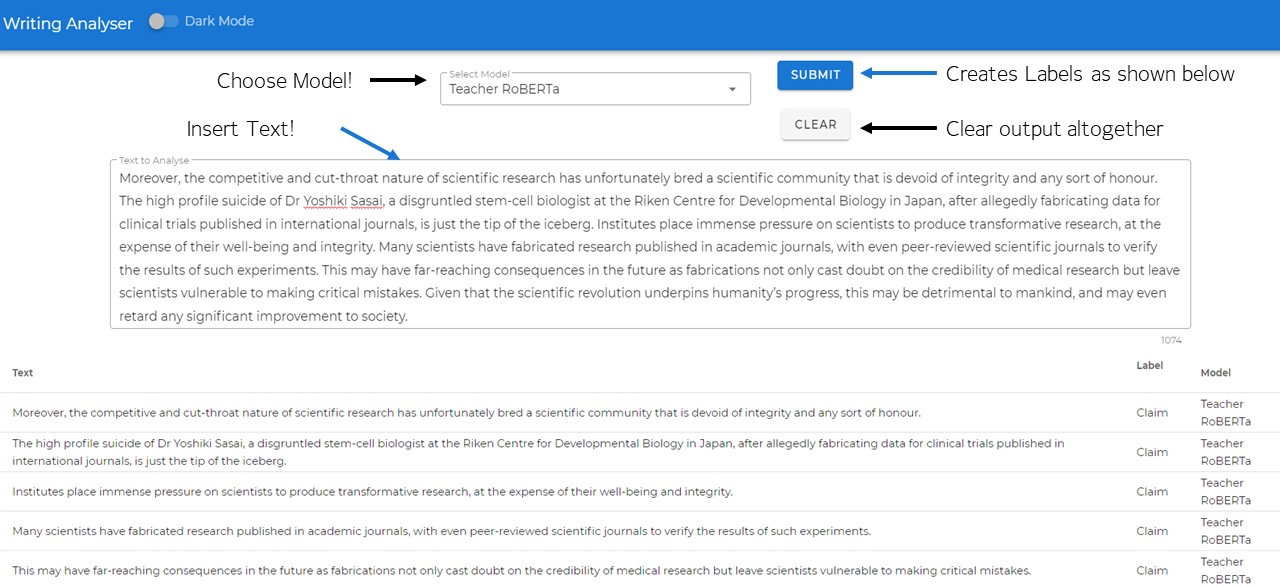
\includegraphics[scale=0.5]{images/userinterface.png}
        \caption{How the User Interface Looks Like.}
        \label{fig:userinterface}
    \end{center}
\end{figure}

\newpage
\section{Results and Conclusion}

% \newpage
\subsection{Teacher Model and Selection}
In this section, we note the results of the Teacher Model Selection. The evaluation metrics considered have been depicted as shown in \textbf{Figure \ref{fig:evalTeacher}}.

\begin{figure}[!h]
    \begin{center}
        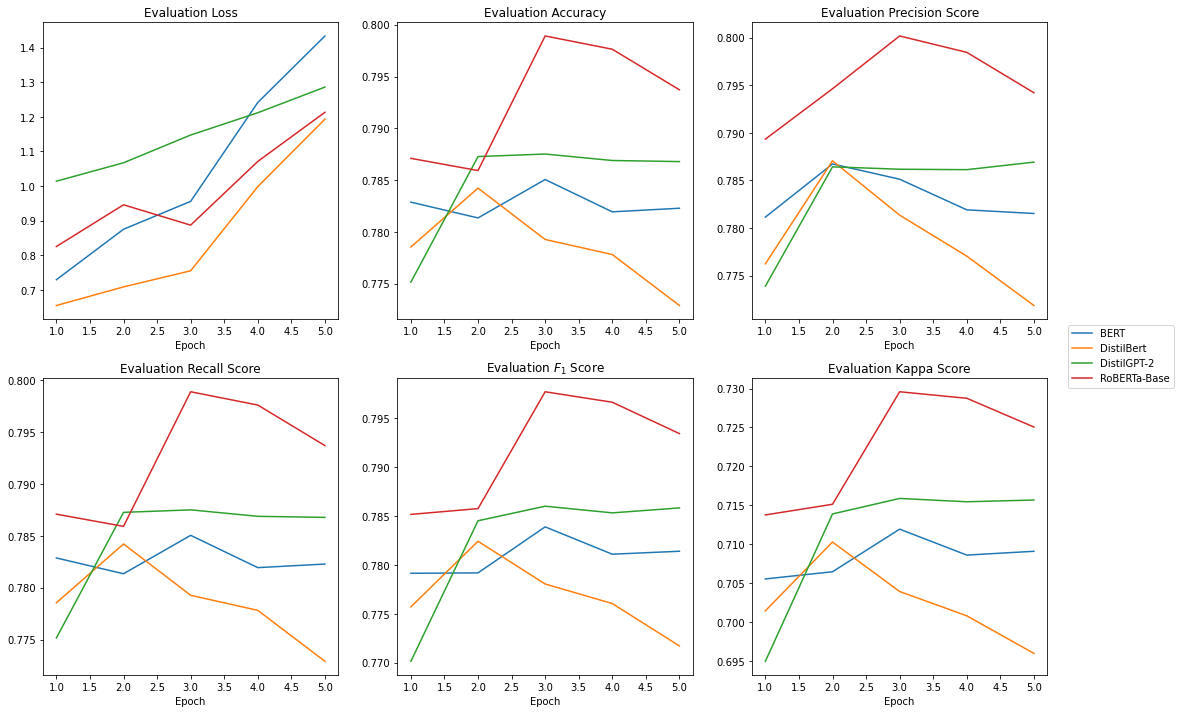
\includegraphics[scale=0.39]{images/metrics.png}
        \caption{Evaluation Metric Values (per Epoch) of each of the Teacher Models.}
        \label{fig:evalTeacher}
    \end{center}
\end{figure}

% \begin{figure}[!h]
%     \begin{center}
%         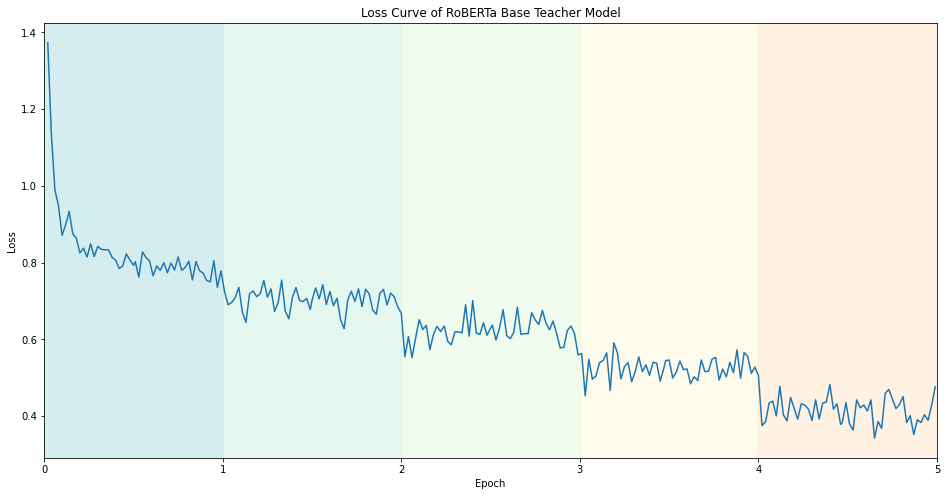
\includegraphics[scale=0.35]{images/robertaloss.png}
%         \caption{The Loss Curve of RoBERTa-Base, our newly identified Teacher Model, as highlighted per epoch.}
%         \label{fig:losscurve}
%     \end{center}
% \end{figure}

Based on our assessments, we have concluded using the best few epochs, based on Validation-based Early Stopping, and hence we produce the data as shown in \textbf{Table \ref{teacherdata}}.

\begin{center}
\begin{tabular}{c c|c c c c c c c}
     Model & Epoch & $\mathcal{L}_{train}$ & $\mathcal{L}_{eval}$ & Accuracy & Precision & Recall & $F_1$ & $\kappa$ \\
     \hline BERT         &      3 &                  0.516 &                 0.956 &     0.785 &      0.785 &   0.785 &  0.784 &     0.712 \\
DistilBERT   &      2 &                  0.469 &                 0.708 &     0.784 &      0.787 &   0.784 &  0.782 &     0.710 \\
DistilGPT-2  &      5 &                  0.837 &                 1.286 &     0.787 &      0.787 &   0.787 &  0.786 &     0.716 \\
RoBERTa-Base &      3 &                  0.619 &                 0.887 &     0.799 &      0.800 &   0.799 &  0.798 &     0.730 \\
\end{tabular}
\captionof{table}{The results of all prospective Teacher Models.}\label{teacherdata}
\end{center}

We note that the \textbf{\texttt{RoBERTa-Base}} model at Epoch \textbf{\texttt{3}} is the best-performing Teacher, hence we decide to continue with this teacher model for our project.


\subsection{Student Model}

\subsubsection{Identifying the best LayerDrop parameter}

To identify the best LayerDrop parameter, we utilise only the New York Times dataset, which is comprised of pseudolabelled New York Times articles, to train 4 different models, each different based on the value $p^*$. The evaluation metrics considered have been depicted as shown in \textbf{Figure \ref{fig:evaluationDropRate}}. Based on the values in Epoch \texttt{5}, we have the following results as shown in \textbf{Table \ref{dropratealtering}}.

\begin{figure}[!h]
    \begin{center}
        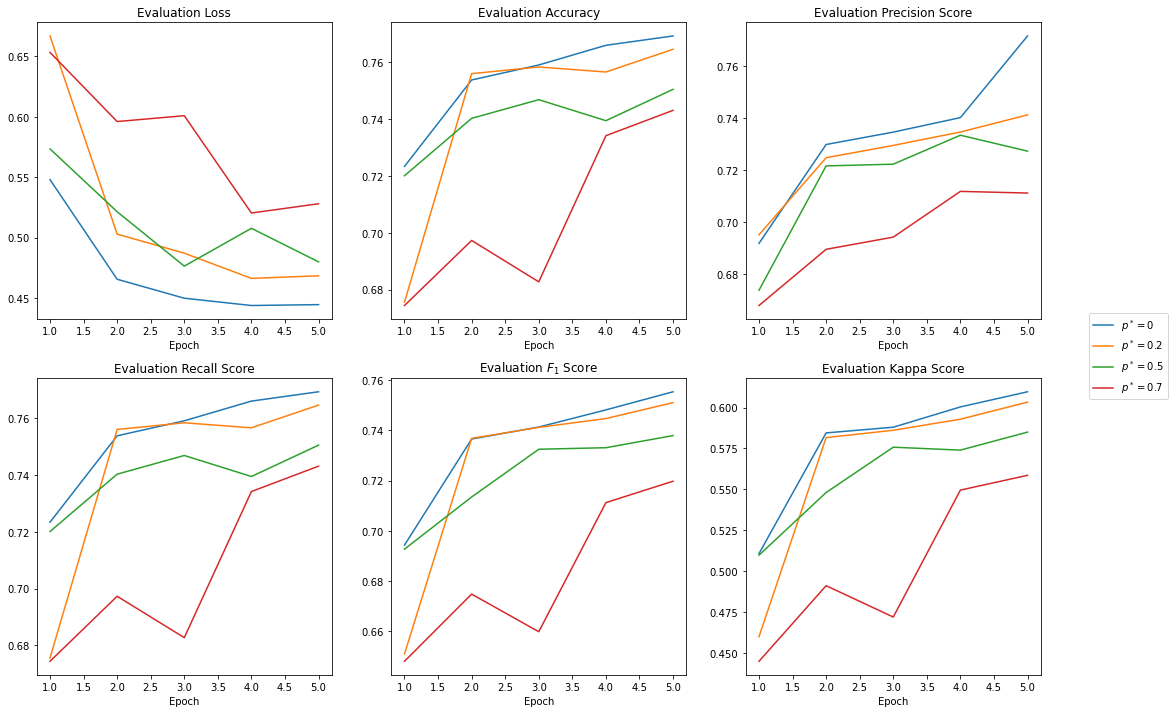
\includegraphics[scale=0.39]{images/metricslayerdrop.png}
        \caption{Evaluation Metric Values (per Epoch) of each of the Student Models, based on their $p^*$ values.}
        \label{fig:evaluationDropRate}
    \end{center}
\end{figure}
\begin{center}
\begin{tabular}{c|c c c c c c c}
     $p^*$ & $\mathcal{L}_{train}$ & $\mathcal{L}_{eval}$ & Accuracy & Precision & Recall & $F_1$ & $\kappa$ \\
     \hline 0 & 0.421 & 0.445 & 0.769 & 0.772 & 0.769 & 0.755 & 0.610 \\
     0.2 & 0.467 & 0.468 & 0.765 & 0.741 & 0.765 & 0.751 & 0.603 \\
     0.3 & 0.373 & 0.495 & 0.780 & 0.768 & 0.780 & 0.770 & 0.616 \\
     0.5 & 0.526 & 0.480 & 0.751 & 0.727 & 0.751 & 0.738 & 0.585 \\
     0.7 & 0.592 & 0.528 & 0.743 & 0.711 & 0.743 & 0.720 & 0.559
\end{tabular}
\captionof{table}{The results of Epoch \texttt{5} based on the different $p^*$ values.}\label{dropratealtering}
\end{center}

While it is clear that Epoch \texttt{5} of the Noisy Student Model with no LayerDrop seems to work the best, we note that $\mathcal{L}_{train} < \mathcal{L}_{eval}$, which indicates a high amount of variance in the dataset, since it seems to overfit on the training set. Hence, we instead use Epoch \textbf{\texttt{5}} of the Noisy Student Model with LayerDrop Rate $\mathbf{p^* = 0.2}$. We also plan to experiment using Epoch \textbf{\texttt{5}} of the Noisy Student Model with LayerDrop Rate $\mathbf{p^* = 0.3}$.

\subsubsection{Identifying the best Iteration}

We now move on to identifying the best iteration, based on our trained student models. Due to time limitations, we only trained 3 iterations, and utilised LayerDrop values  of $p^* \in \{0.2, 0.7\}$, as was concluded in the previous section. The evaluation metrics considered have been depicted as shown in \textbf{Figure \ref{fig:evaluationIters}}. This gave us a good understanding of the iteration process. Based on the values in Epoch \texttt{5}, we have the following results as shown in \textbf{Table \ref{iterationdata}}.

\begin{figure}[!h]
    \begin{center}
        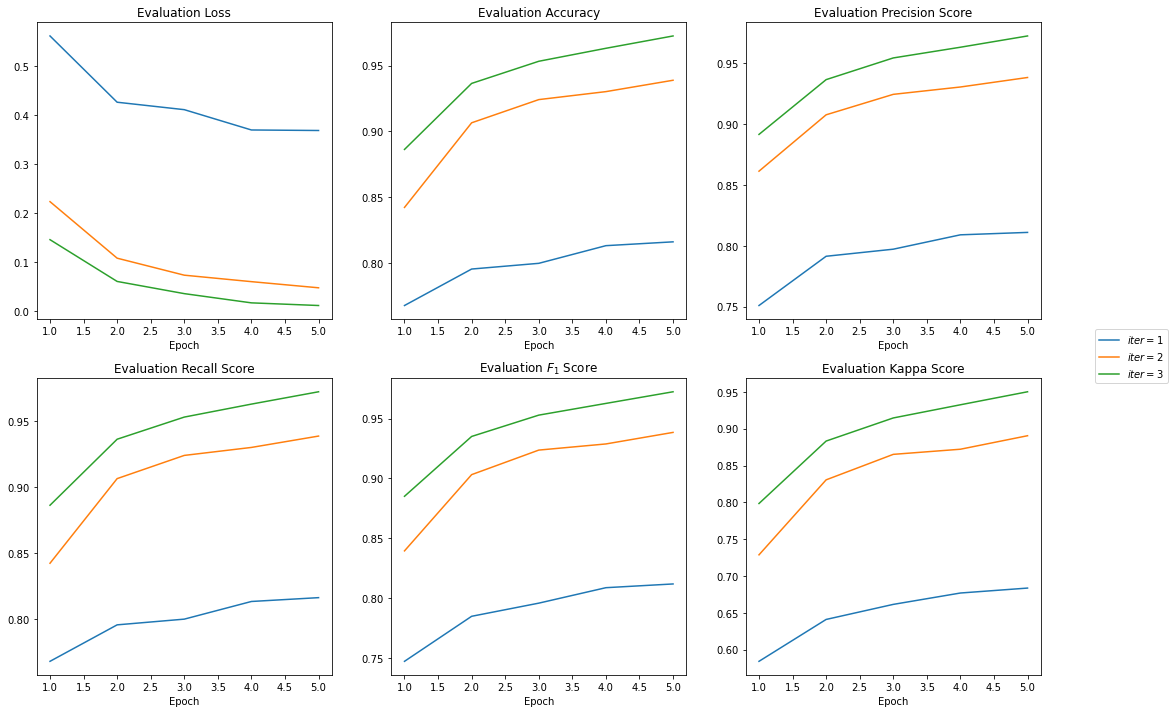
\includegraphics[scale=0.39]{images/metricsiters.png}
        \caption{Evaluation Metric Values (per Epoch) of each of the Student Models, across different iterations ($p^* = 0.2$).}
        \label{fig:evaluationIters}
    \end{center}
\end{figure}

\begin{center}
\begin{tabular}{c|c c c c c c c}
Iteration & $\mathcal{L}_{train}$ & $\mathcal{L}_{eval}$ & Accuracy & Precision & Recall & $F_1$ & $\kappa$ \\
\hline 1 & 0.446 & 0.369 & 0.816 & 0.811 & 0.816 & 0.812 & 0.684 \\
2 & 0.159 & 0.047 & 0.939 & 0.938 & 0.939 & 0.938 & 0.890 \\
3 & 0.145 & 0.011 & 0.972 & 0.973 & 0.972 & 0.972 & 0.950 \\
\end{tabular}
\captionof{table}{The results of Epoch \texttt{5} across different iterations ($p^* = 0.2$).}\label{iterationdata}
\end{center}

It can be clearly seen that the performance of the model improves with each iteration of the teacher student model training, and hence the ideal iteration count, in this case, for Noisy Student Training is the \textbf{3rd Iteration}.

\subsection{Pruning of Student Models}
We used a student model with pruning value of $p^*=0.7$ so as to showcase the results of pruning at the most extreme values. Following the "every other" pruning method suggested by Fan et al.\cite{layerdrop}, we simply drop every layer at depth $d$ where $d=k(\frac{1}{p})$ where $k$ is an arbitrary integer. The results are as described in \ref{fig:pruning}.

\begin{figure}[!ht]
    \begin{center}
        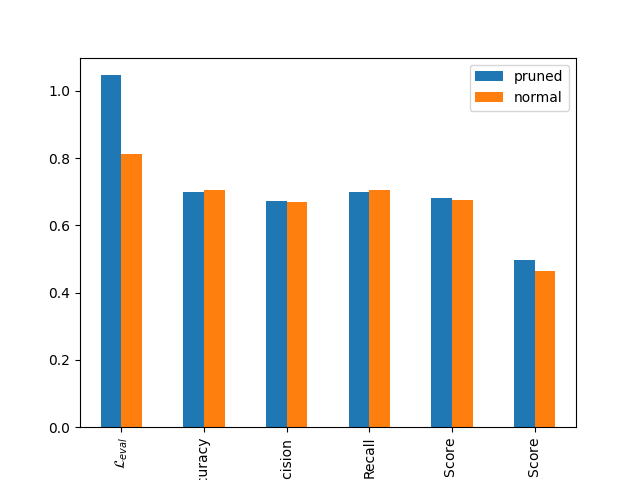
\includegraphics[scale=0.6]{images/prunedShow.png}
        \caption{How Pruning Helps.}
        \label{fig:pruning}
    \end{center}
\end{figure}

As we can see, there is not a significant drop in performance for the pruned model in all metrics other than loss, and in fact the pruned model has a parameter count more than 26 times smaller than the normal model. 

\section{Conclusion}
One thing to note in the above sections is that the metrics computed are based off the labels of the previous teacher model. In order to conclude that the model has actually improved in performance, we compare the model's performance to our labelled Feedback Prize dataset(\ref{section:feedbackprize}) and a subset of manually labelled New York Times Dataset(\ref{section:nytimes}) articles, as depicted in \textbf{Table \ref{feedbackprizecomp}}.
\begin{center}
\begin{tabular}{c|c c c c}
Metric & $\mathcal{M}_{teacher}$ & $\mathcal{M}_{student, 0}$ & $\mathcal{M}_{student, 1}$ & $\mathcal{M}_{student, 2}$ \\
\hline Accuracy & 0.860 & 0.740 & 0.730 & 0.726 \\
Mean IoU & 0.695 & 0.491 & 0.480 & 0.482 \\
Weighted Precision Score & 0.863 & 0.753 & 0.744 & 0.746 \\
Weighted Precision Score & 0.863 & 0.753 & 0.744 & 0.746 \\
$\kappa$ Score & 0.811 & 0.641 & 0.627 & 0.622 \\
Weighted $F_1$ Score & 0.858 & 0.732 & 0.721 & 0.718 \\
\end{tabular}
\captionof{table}{Comparison of multiple metrics between the models ($p^* = 0.2$) on the Feedback Prize dataset.}\label{feedbackprizecomp}
\end{center}

This result is not ideal, as we can see that for every score, the value has dropped significantly in the cases of any $M_{student, i}$. This is unideal, and although the comparison over the teacher model bore positive results for these models, we must unfortunately conclude that Noisy Student Training does not perform well, nor improve the scores of the models.

However, after running and evaluating a separate model run for 15 epochs, we reached much higher values for these metrics, which suggests that our models did not train for enough epochs, and are possibly undertrained, thus further improvement can be made for the model to ensure that the accuracy improves.

\section{Discussion and Future Work}

\subsection{Novelty of Methods used}

In our project, we utilised Noisy Student Training, an algorithm traditionally used in Image Processing and Computer Vision tasks, on a Natural Language Processing (NLP) task, which made this task all the more novel. Whilst this sort of training has been performed before on NLP tasks, it has been relatively scarce, and our work, albeit showing negative results, is a testament to how this technique is still relatively usable in other fields other than Computer Vision, although it may not bear the monumental results achieved in Xie et al~\cite{noisystudent}.

\subsection{Technical and Conceptual Limitations}

One of the main limitations in this project was the limited amount of processing power and time, since only one of possessed GPUs. Even if we had used Google Colaboratory, the training time, in addition to preprocessing and acquisition, would not be able to sustain the duration as configured in the free version. Due to monetary limitations, we did not proceed to purchase licenses for AWS SageMaker of Google Colaboratory Pro, which would have definitely helped in speeding up this project.

In terms of conceptual limitations, this was our first Natural Language Processing (NLP) project, and even though one of us had delved into Topic Modelling before, this was a much more complex project for us to tackle, especially given the lack of topical info taught in the module with regards to NLP. This indeed posed a challenge for us, since the documentation for HuggingFace was not that great, and understanding Transformers was a bit difficult with all of this novel research, of sorts.

\subsection{Future Work}
Our current model does not use the influence of other textual elements around the sentence to change the decision of the model, which can be solved if we use Sequential Sentence Classification (SSC)\cite{SSC}, which allows us make sentence classifications based on the surrounding local context, which would likely improve our classification accuracies as many labels are dependent on the content of the previous and next sentences.

Another interesting exploration would be the usage of alternative sentence augmentation techniques. In our project, we decided to dial down to abstractive summarisation methods over a subset of our data due to time considerations, but realistically more noise can be added to the dataset to ensure greater robustness against noisy samples.

Additionally, we could explore the possibly of text style transfer~\cite{styletransfersurvey,deeplearningtextstyletransfer}, training a model to convert from informal to formal writing or vice versa, as the styles of the two datasets that we used varied vastly due to the nature of how the data was obtained, and this would have been an interesting avenue of exploration.

\newpage
\section{Reflection}

\subsection{Wei Pyn}
Through the course of the project I learnt a lot more about transformers and implementation of large libraries, having to subclass and look through the source code of the HuggingFace library to implement the Noisy Student architecture. I believe that if we had more time, we could possibly perfect the process and more thoroughly explore the possibilities. Perhaps we did not properly train the teacher model for enough epochs, and that lead to the slow degradation of student model quality with each iteration, although that is left to future work.

\subsection{Prannaya}
In this project, I worked on many things that I had never even learnt before, such as transformers and novel techniques such as noisy student training and knowledge distillation. These have helped me gain a greater appreciation over the way that AI infrastructure is usually handled, and I am more motivated to pursue AI research in the future. While the task itself was relatively challenging, I think with the time that we have gotten, we achieved the best that we could. With more time, we could have certainly done a brilliant project, but even as it stands, I think we have achieved what we aimed for, and that, I believe, is what makes our project good. As for what I learnt, I think we both have worked through a lot of struggles and for me, that was the User Interface, which was difficult to format given my limited understanding of Flask and only recent introduction to Vue as part of AppVenture. However, I think this has given me a great purview into how many companies automate AI-powered websites.

\section{Work Distribution Matrix}
\begin{center}
\begin{tabular}{|c|c|c|}
    \hline
    & Prannaya & Wei Pyn \\ [0.5ex] 
    \hline\hline
    Project Brainstorm and Planning & \checkmark & \checkmark \\
    Dataset Sourcing and Acquisition & \checkmark &  \\
    Data Cleaning and Preprocessing & \checkmark & \checkmark \\
    Training Teacher Models &  & \checkmark  \\
    Pseudo-Labelling and Noise Injection & \checkmark & \checkmark \\
    Training Student Model & & \checkmark \\
    User Interface (UI) & \checkmark &  \\
    Presentation Slides & \checkmark & \checkmark \\
    Report Writing & \checkmark & \checkmark \\
    Video Presentation & \checkmark & \checkmark \\
    \hline
\end{tabular}
\end{center}


\newpage


\section{References}

\printbibliography[
heading=none
]
}

\end{document}